\section{Centered-square results}
\label{app:square}

Table~\ref{tab:square_fusion_full} separates the velocity and pressure errors
for the joint-field comparison in Table~\ref{tab:routing_fusion}. Best single
in the main text means one fixed specialist per overlap, chosen for comparison
by the lowest aggregate joint error: Hopf for $S$--$H$ and Periodic for $H$--$P$.
It is distinct from the window-wise convex oracle, which uses the reference
solution to choose a weight for each evaluation window.

\paragraph{Overlap evaluation and descriptor ablation.}
The routing/fusion errors $E_u$, $E_p$, and $E_{\mathrm{joint}}=E_u+E_p$ are
terminal-step ($k=24$) errors averaged over 16 held-out windows per overlap.
Each of the two held-out Reynolds numbers contributes eight windows, so the
pooled window mean equals the mean of the per-$Re$ window averages. This
terminal metric is distinct from the full-window mean used by the oracle
(Appendix~\ref{app:routing}). T2-C $\mu$-only retains the correction network,
parameter count, training/validation partitions, optimizer, and selection
rule, but sets all standardized history-descriptor channels to zero.
Table~\ref{tab:square_fusion_full} retains the original fixed-run comparisons
and adds the $\mu$-only run with seed 42001; seed averages are reported separately.

\begin{table}[!htbp]
\centering
\caption{Complete centered-square routing and fusion errors at $K=24$.
All errors are percentages. The convex oracle is an a posteriori reference;
bold marks the best deployable assembly for each field metric.
T2-C $\mu$-only zeroes standardized history channels without changing the gate architecture.}
\label{tab:square_fusion_full}
\small
\setlength{\tabcolsep}{5pt}
\begin{tabular}{@{}llrrr@{}}
\toprule
Overlap & Predictor & $E_u$ & $E_p$ & $E_{\mathrm{joint}}$ \\
\midrule
$S$--$H$ & Steady specialist & 2.5976 & 2.2450 & 4.8426 \\
 & Hopf specialist & 0.4942 & 1.2356 & 1.7298 \\
 & E2 Top-1 & 0.4942 & 1.2356 & 1.7298 \\
 & Equal blend & 1.3644 & 1.6677 & 3.0321 \\
 & E2-probability blend & 0.7898 & 1.3949 & 2.1847 \\
 & T2-C $\mu$-only & 0.7898 & 1.3948 & 2.1846 \\
 & T2-C & \textbf{0.4615} & \textbf{0.7343} & \textbf{1.1958} \\
 & Convex oracle & 0.4659 & 0.7183 & 1.1842 \\
\midrule
$H$--$P$ & Periodic specialist & 0.6420 & 0.5659 & 1.2079 \\
 & Hopf specialist & 1.0034 & 1.8684 & 2.8718 \\
 & E2 Top-1 & 0.7422 & 1.1052 & 1.8473 \\
 & Equal blend & 0.6077 & 1.0069 & 1.6146 \\
 & E2-probability blend & 0.6154 & 1.0464 & 1.6618 \\
 & T2-C $\mu$-only & 0.5875 & 0.5629 & 1.1504 \\
 & T2-C & \textbf{0.4509} & \textbf{0.3956} & \textbf{0.8465} \\
 & Convex oracle & 0.4479 & 0.3905 & 0.8384 \\
\bottomrule
\end{tabular}
\end{table}

\begin{table}[!htbp]
\centering
\caption{Parameter-wise centered-square routing and T2-C results at $K=24$.
Joint errors and relative error reductions are percentages. The mean weight
is the steady weight for $S$--$H$ and the periodic weight for $H$--$P$.}
\label{tab:square_parameter}
\small
\setlength{\tabcolsep}{3.5pt}
\begin{tabular}{lrlrrrr}
\toprule
Overlap & $Re$ & E2 choice & $\bar\alpha$ & E2 $E_{\mathrm{joint}}$ & T2-C $E_{\mathrm{joint}}$ & Reduction \\
\midrule
$S$--$H$ & 95.1 & Hopf & 0.0967 & 1.7140 & 1.1827 & 31.00\% \\
$S$--$H$ & 95.3 & Hopf & 0.0971 & 1.7456 & 1.2090 & 30.74\% \\
$H$--$P$ & 100.5 & Hopf & 0.5870 & 2.6485 & 0.8571 & 67.64\% \\
$H$--$P$ & 102.0 & Periodic & 0.7094 & 1.0462 & 0.8360 & 20.09\% \\
\bottomrule
\end{tabular}
\end{table}

The aggregate local-specialist errors are $(E_u,E_p)=(1.5311,1.4583)\%$ for steady flow, $(0.4387,0.4844)\%$ for Hopf-onset flow, and $(0.9395,1.0921)\%$ for periodic flow. On the aggregate $S$--$H$ evaluation, the steady and Hopf specialists have joint errors $4.8426\%$ and $1.7298\%$; on $H$--$P$, the periodic and Hopf specialists give $1.2079\%$ and $2.8718\%$. These results show why the best local choice can change between overlaps and why a corrected convex assembly is useful.

\FloatBarrier
\paragraph{Gate-training seed variability.}
Only the lightweight gate is retrained for seeds 42001, 42002, and 42003.
Specialists, E2, candidate rollouts, partitions, normalization, and optimization
settings are fixed. Both modes use AdamW (learning rate $3\times10^{-4}$,
weight decay $10^{-4}$), 8,000 steps, and gradient-norm clipping at 1.
Minibatches sample training windows with replacement. Validation is evaluated
at step 1 and every 100 steps; the selected model minimizes the worst-$Re$
full-window mean joint error, then the pooled mean, without test-based selection.
Table~\ref{tab:t2c_seed_variability} reports mean and sample standard deviation
($N=3$, denominator $N-1$); this is gate-seed variability, not across-$Re$
variation, a confidence interval, or full-pipeline uncertainty.
Table~\ref{tab:t2c_seedwise} gives individual joint errors.

\begin{table}[!htbp]
\centering
\caption{Three-seed variability of the centered-square T2-C gate at the K24
terminal step. Values are percentages, mean $\pm$ sample SD across gate-training
seeds, conditional on fixed specialists, E2, candidate rollouts, partitions,
and normalization. Bold marks the lower mean within each overlap.}
\label{tab:t2c_seed_variability}
\small
\setlength{\tabcolsep}{4pt}
\begin{tabular}{@{}llccc@{}}
\toprule
Overlap & Gate & $E_u$ & $E_p$ & $E_{\mathrm{joint}}$ \\
\midrule
$S$--$H$ & T2-C $\mu$-only & $0.79006\pm0.00026$ & $1.39498\pm0.00012$ & $2.18504\pm0.00038$ \\
 & Full T2-C & $\mathbf{0.46156\pm0.00004}$ & $\mathbf{0.73416\pm0.00014}$ & $\mathbf{1.19572\pm0.00010}$ \\
\midrule
$H$--$P$ & T2-C $\mu$-only & $0.59067\pm0.00461$ & $0.56050\pm0.00435$ & $1.15116\pm0.00070$ \\
 & Full T2-C & $\mathbf{0.45211\pm0.00138}$ & $\mathbf{0.39793\pm0.00215}$ & $\mathbf{0.85004\pm0.00347}$ \\
\bottomrule
\end{tabular}
\end{table}

\begin{table}[!htbp]
\centering
\caption{Seed-wise centered-square K24 terminal $E_{\mathrm{joint}}$ (\%).
Each column uses the same training seed for both gate variants.}
\label{tab:t2c_seedwise}
\small
\begin{tabular}{@{}llrrr@{}}
\toprule
Overlap & Gate & 42001 & 42002 & 42003 \\
\midrule
$S$--$H$ & T2-C $\mu$-only & 2.18460 & 2.18524 & 2.18527 \\
 & Full T2-C & 1.19584 & 1.19567 & 1.19565 \\
\midrule
$H$--$P$ & T2-C $\mu$-only & 1.15037 & 1.15170 & 1.15143 \\
 & Full T2-C & 0.84653 & 0.85011 & 0.85348 \\
\bottomrule
\end{tabular}
\end{table}

Full T2-C improves upon $\mu$-only for all three paired seeds in both overlaps;
the reductions in three-seed mean joint error are $45.28\%$ ($S$--$H$) and
$26.16\%$ ($H$--$P$). The $S$--$H$ $\mu$-only runs all select step 1 after
completing 8,000 training steps: later models do not improve the prescribed
validation criterion. They remain close to direct probability blending.
The $H$--$P$ $\mu$-only runs select step 400 and improve that baseline.
These observations support history conditioning under the tested protocol,
not a universal limitation of parameter-only correction.

\FloatBarrier
Figures~\ref{fig:app_square_sh_full} and \ref{fig:app_square_hp_full}
provide the complete velocity, gauge-corrected pressure, and pointwise-error
views underlying the compact main-text comparison.

\begin{figure}[p]
\centering
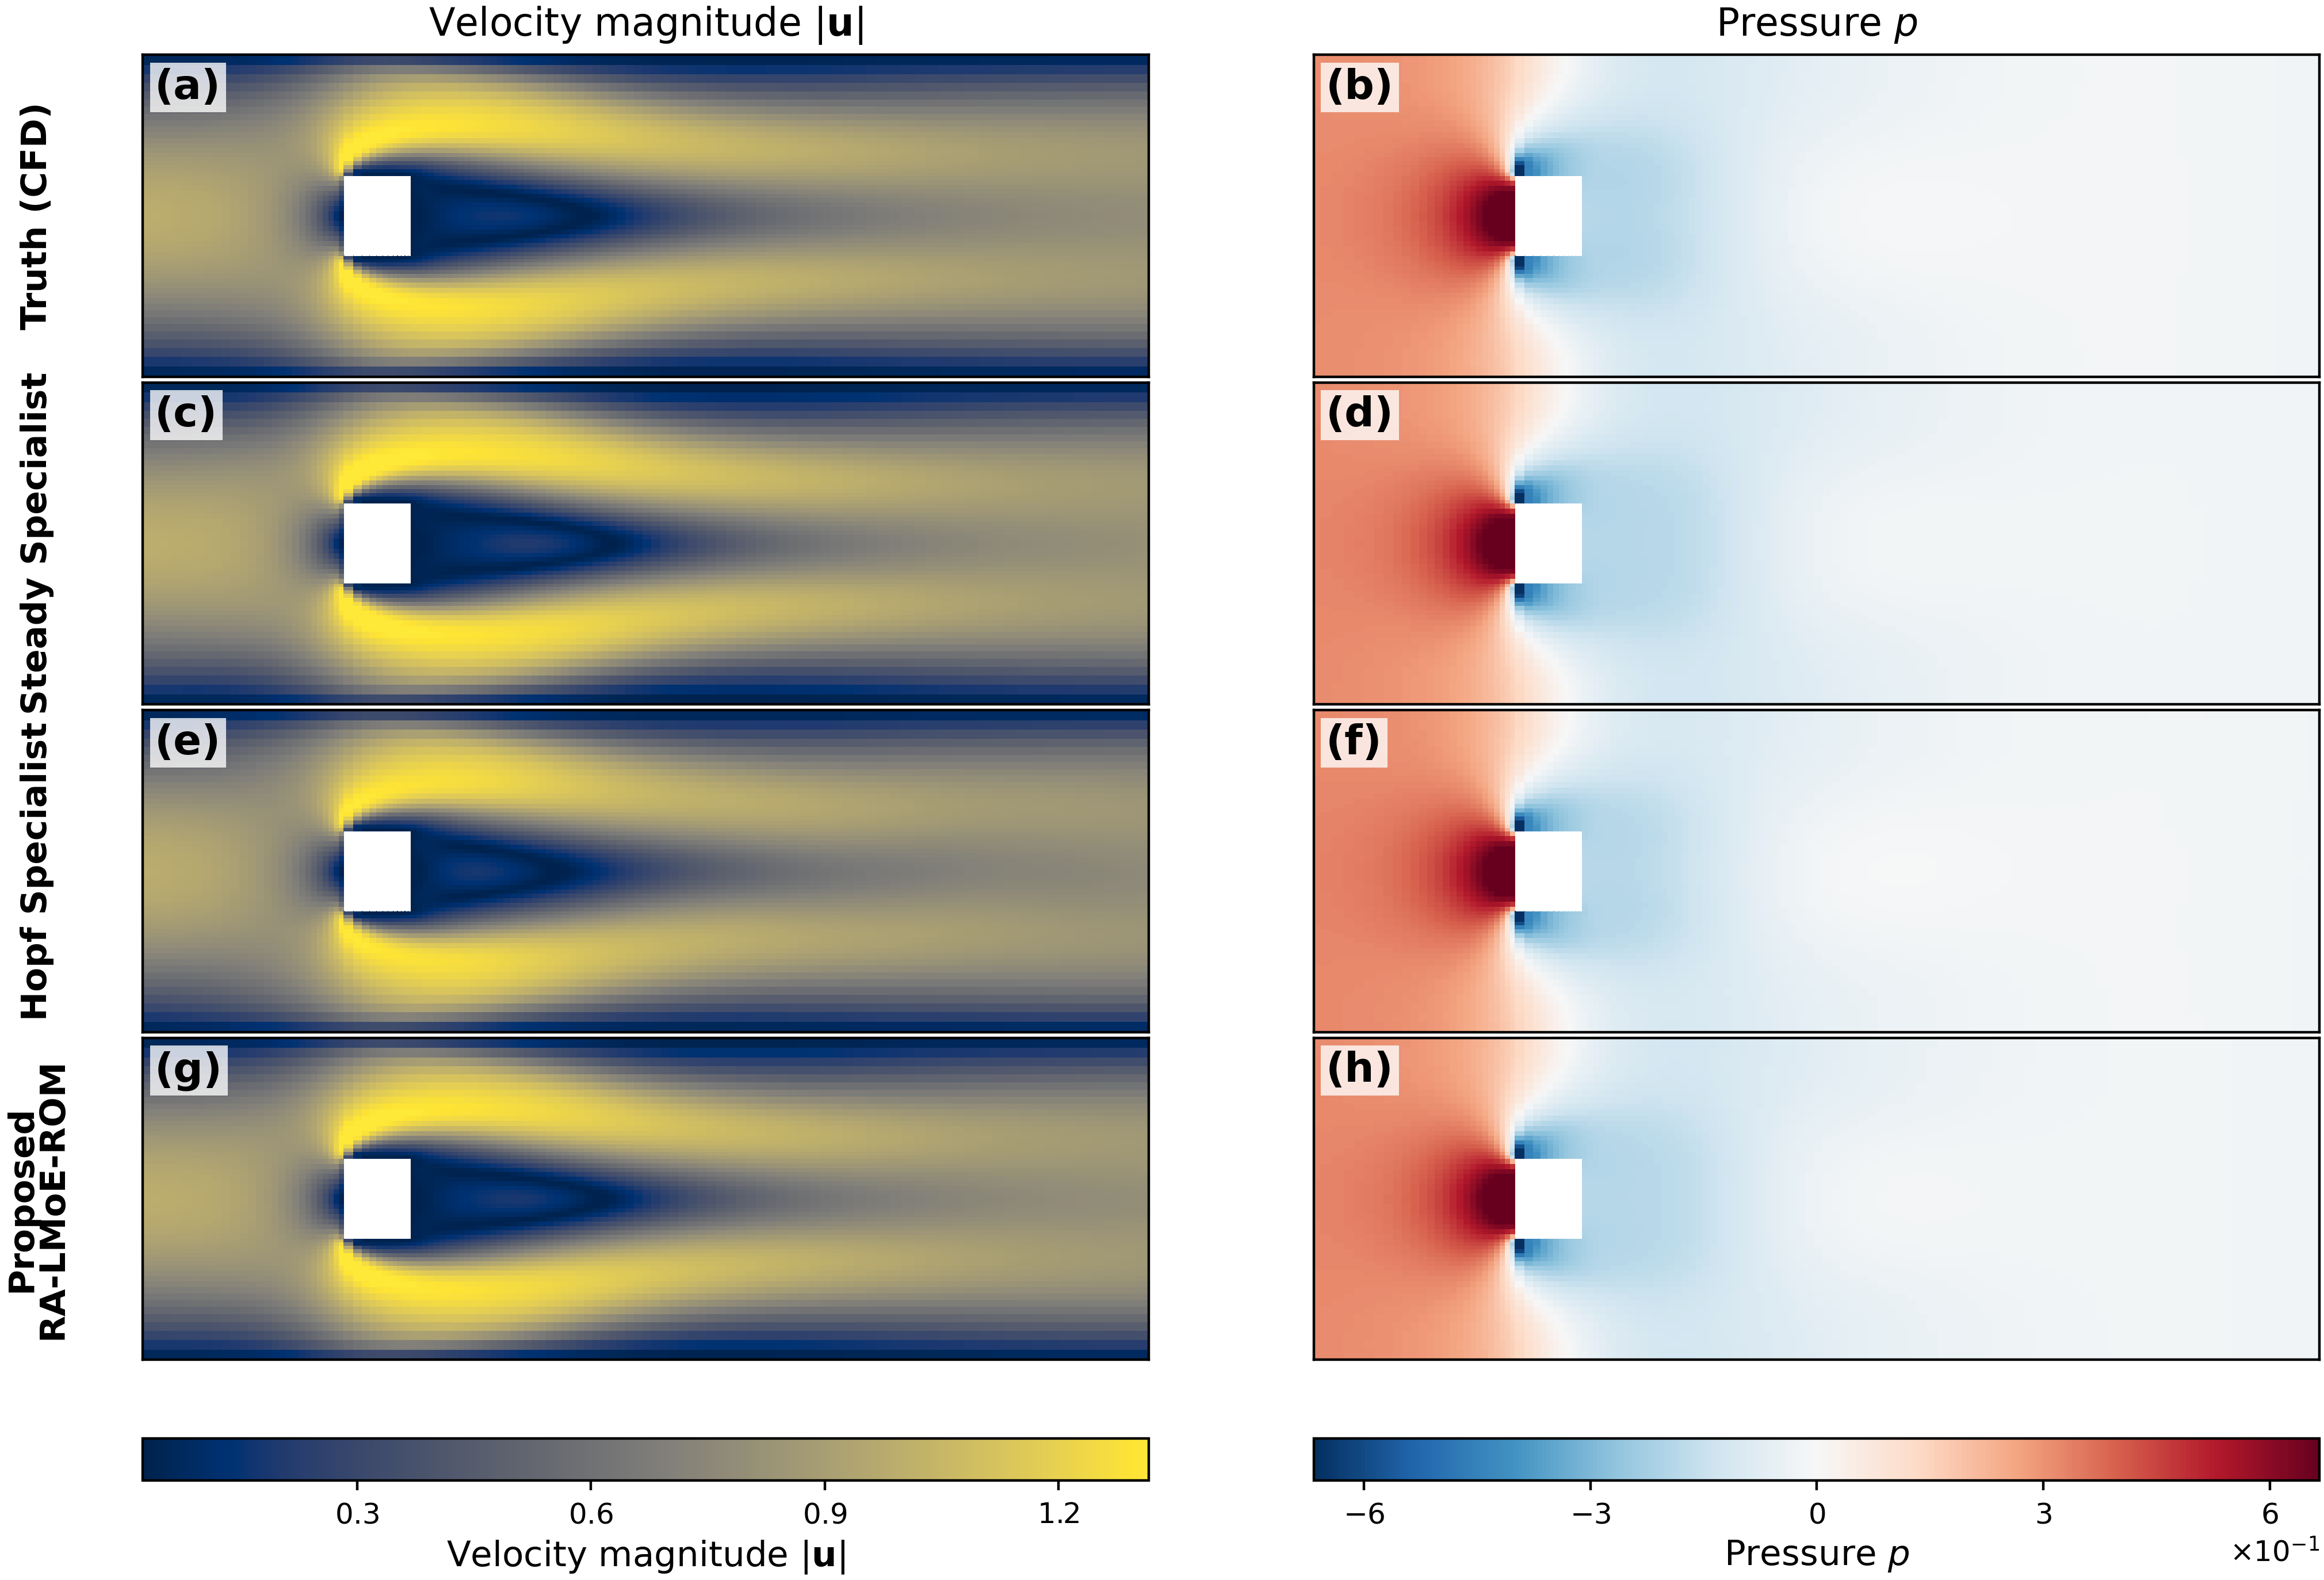
\includegraphics[width=0.80\linewidth]{figures/original/SH_2.png}

\vspace{0.35em}
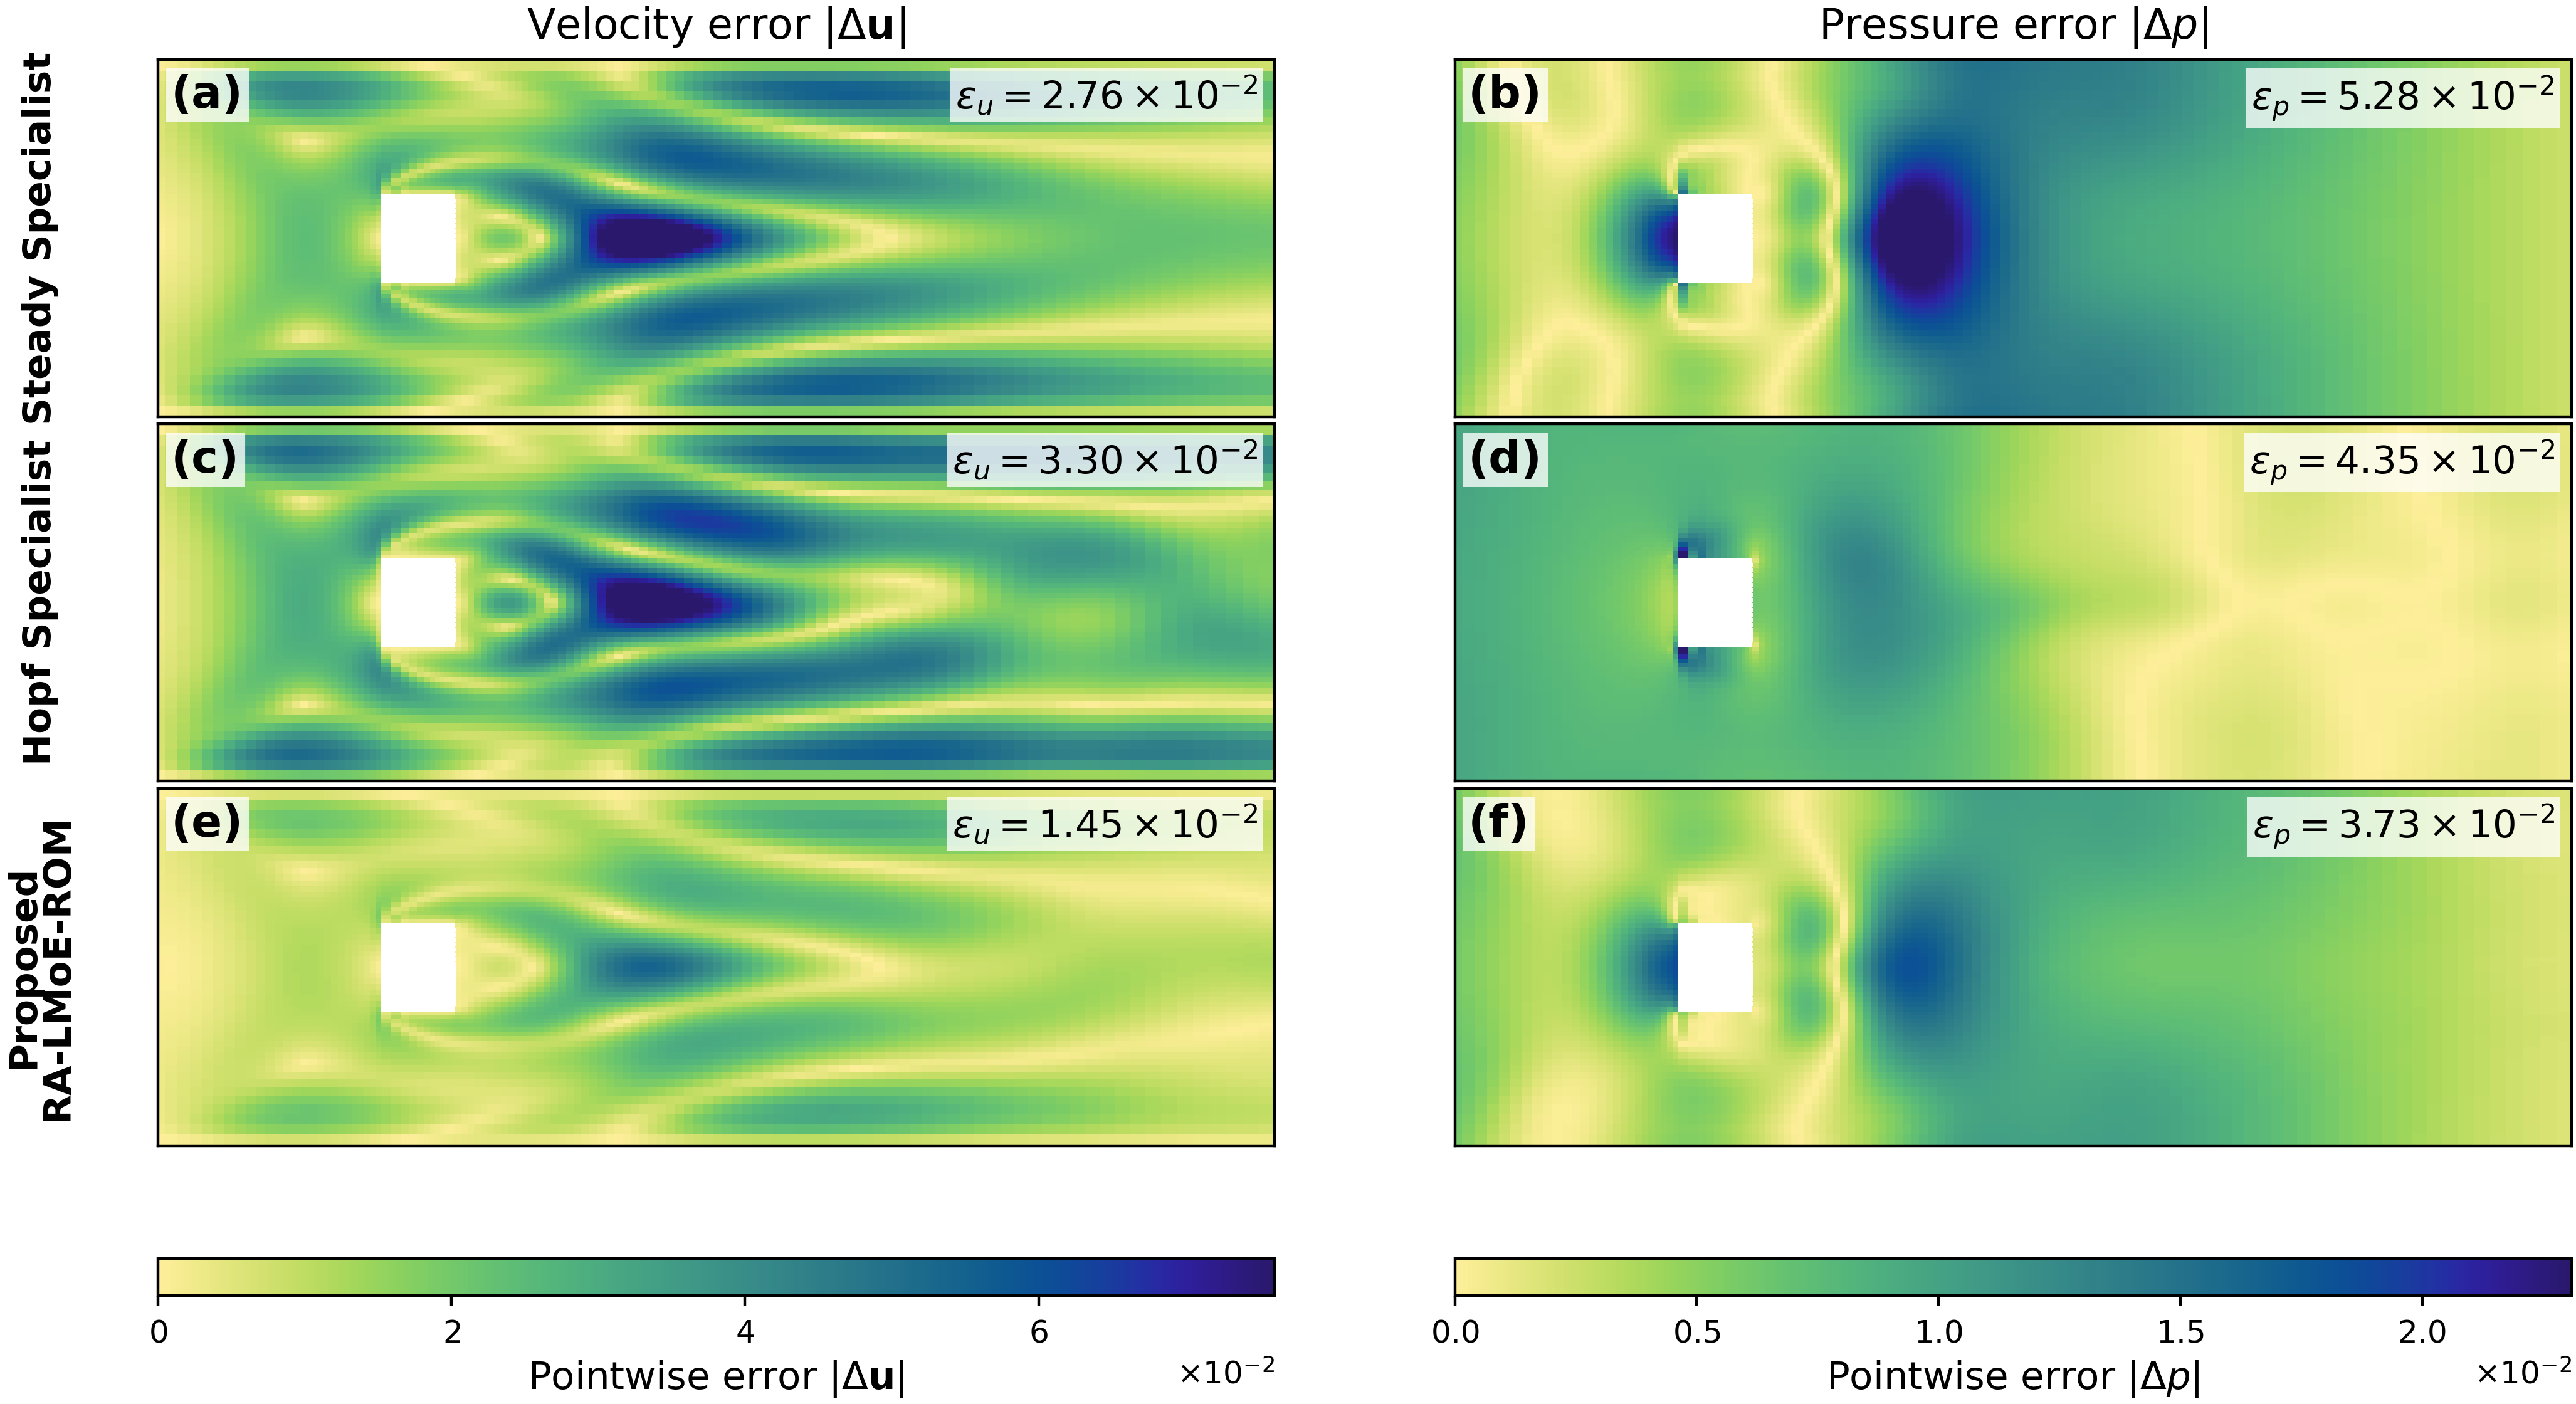
\includegraphics[width=0.80\linewidth]{figures/original/SH_2_1.png}
\caption{Representative held-out prediction in the centered-square
$S$--$H$ overlap at $Re=95.1$. The upper panel compares the CFD reference,
Steady specialist, Hopf specialist, and T2-C prediction for velocity
magnitude and gauge-corrected pressure. The lower panel gives the
corresponding pointwise absolute errors.}
\label{fig:app_square_sh_full}
\end{figure}

\begin{figure}[p]
\centering
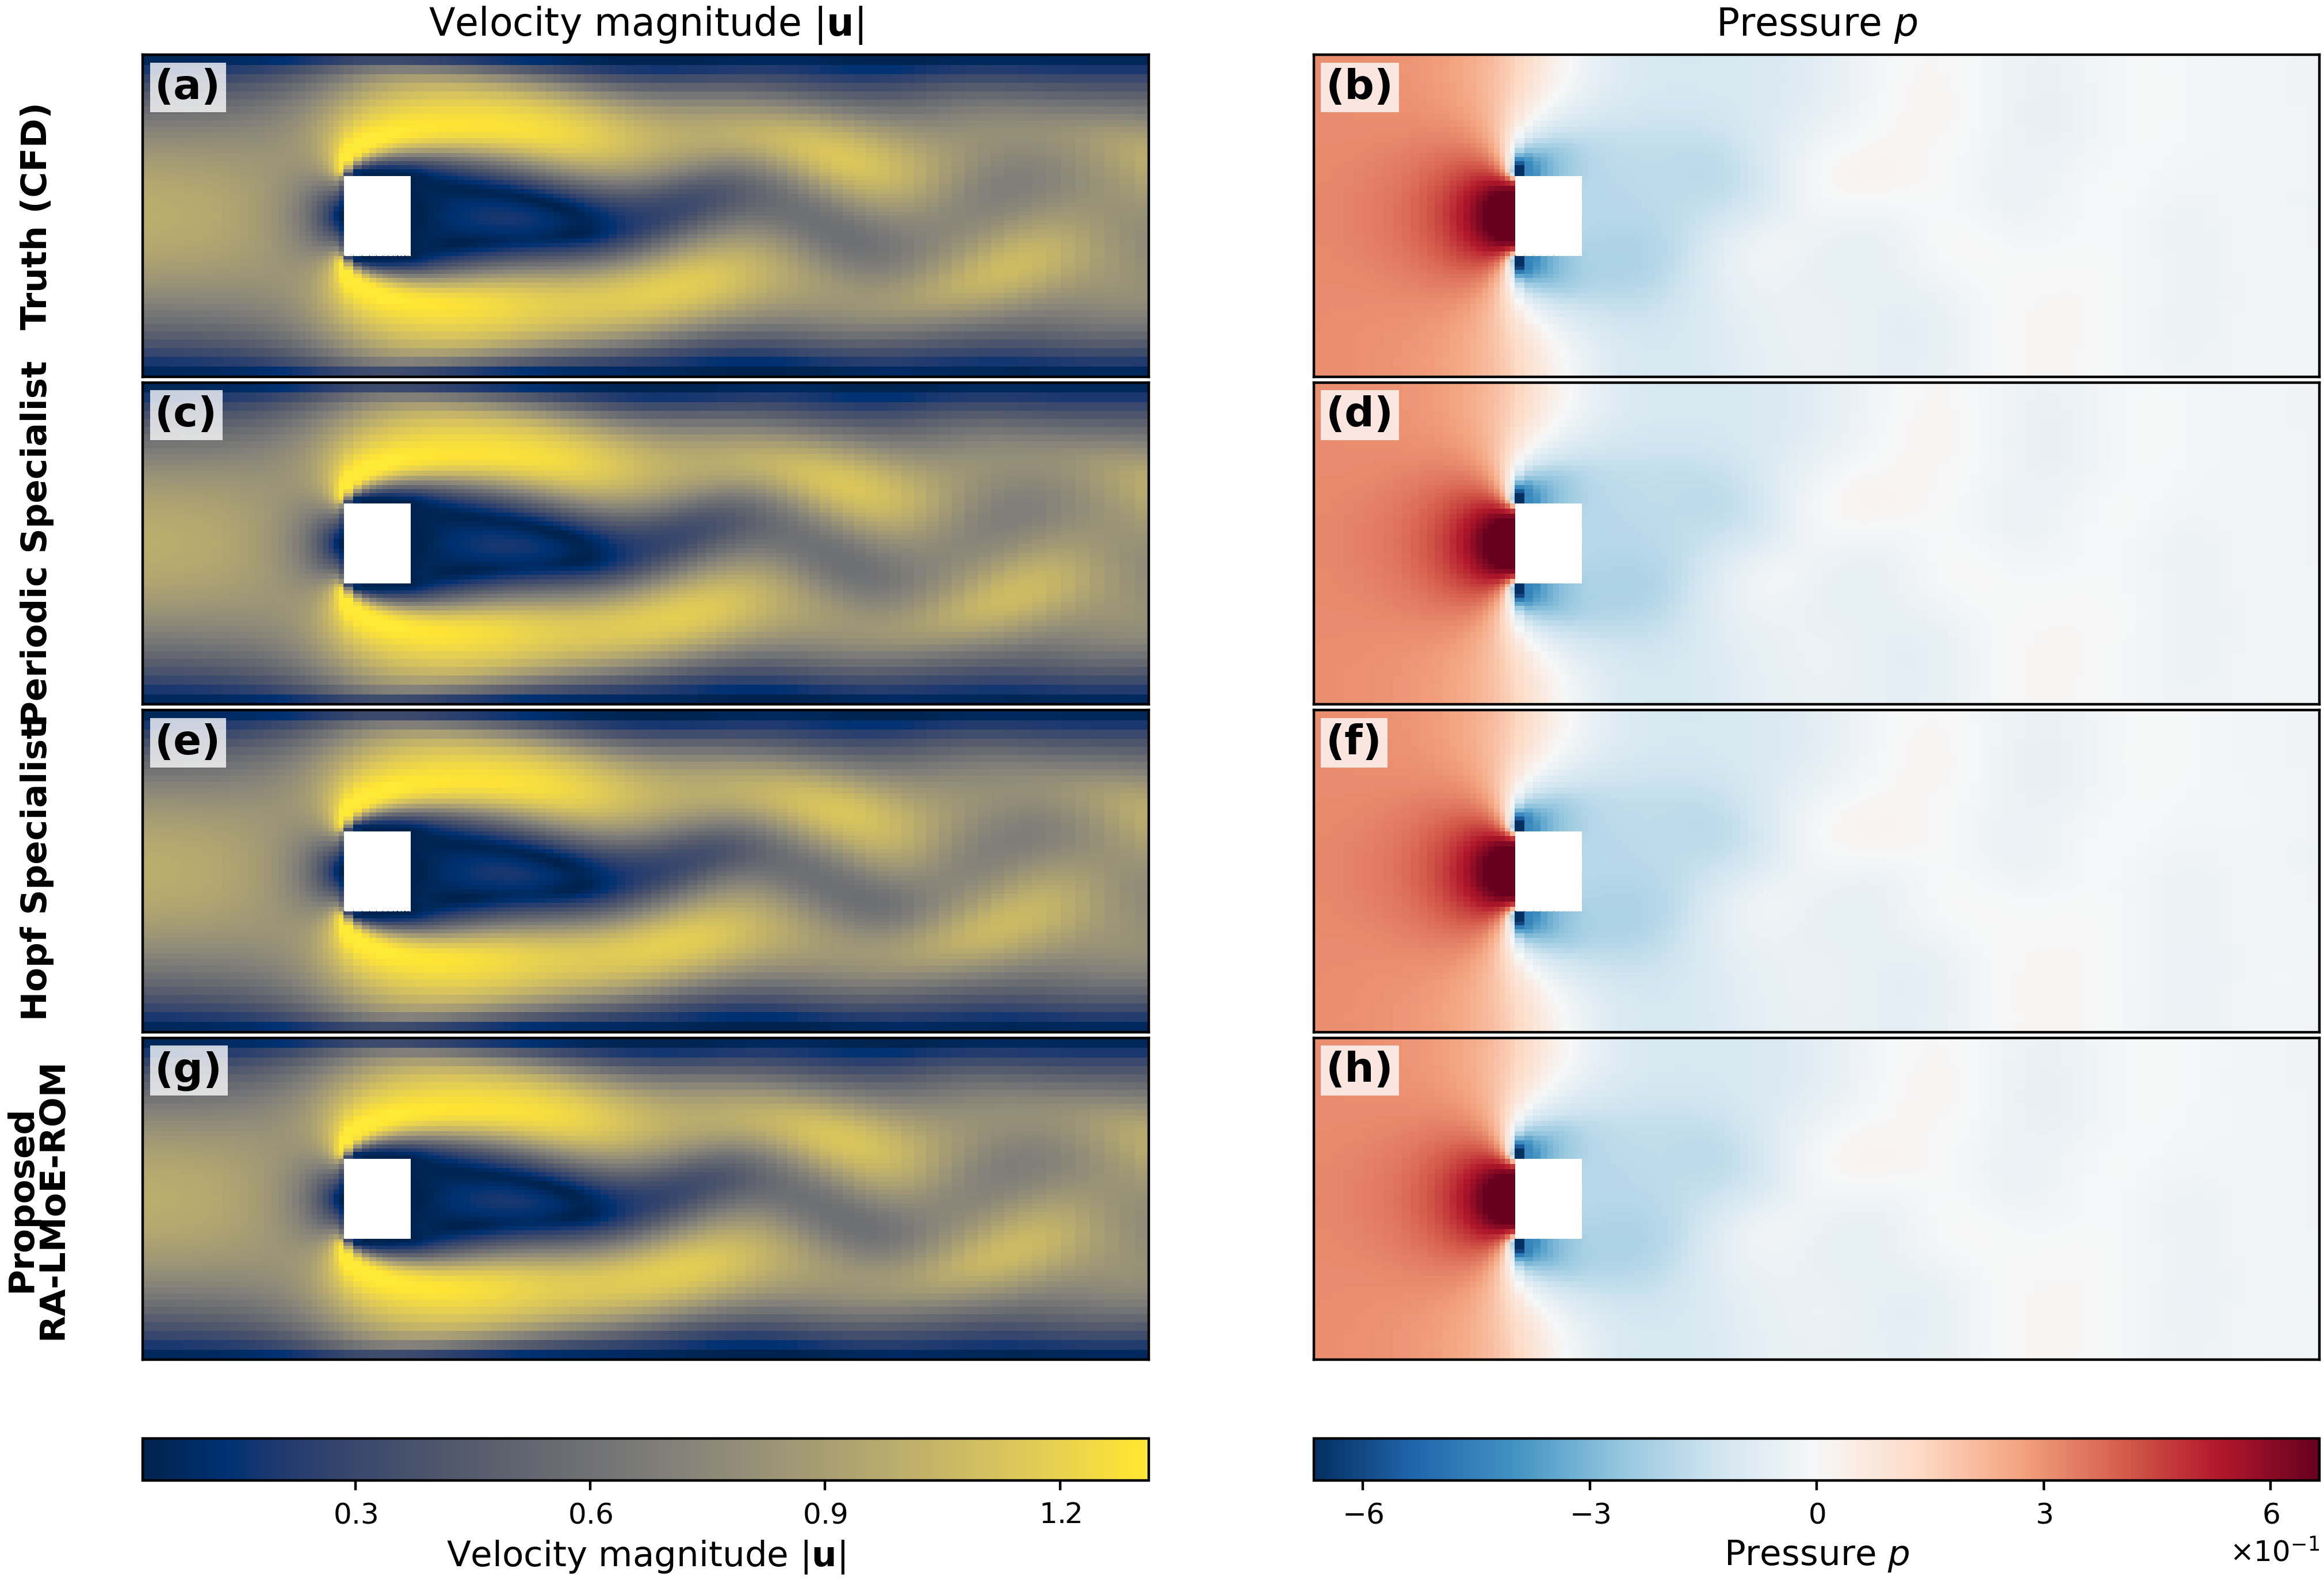
\includegraphics[width=0.80\linewidth]{figures/original/HP_2.png}

\vspace{0.35em}
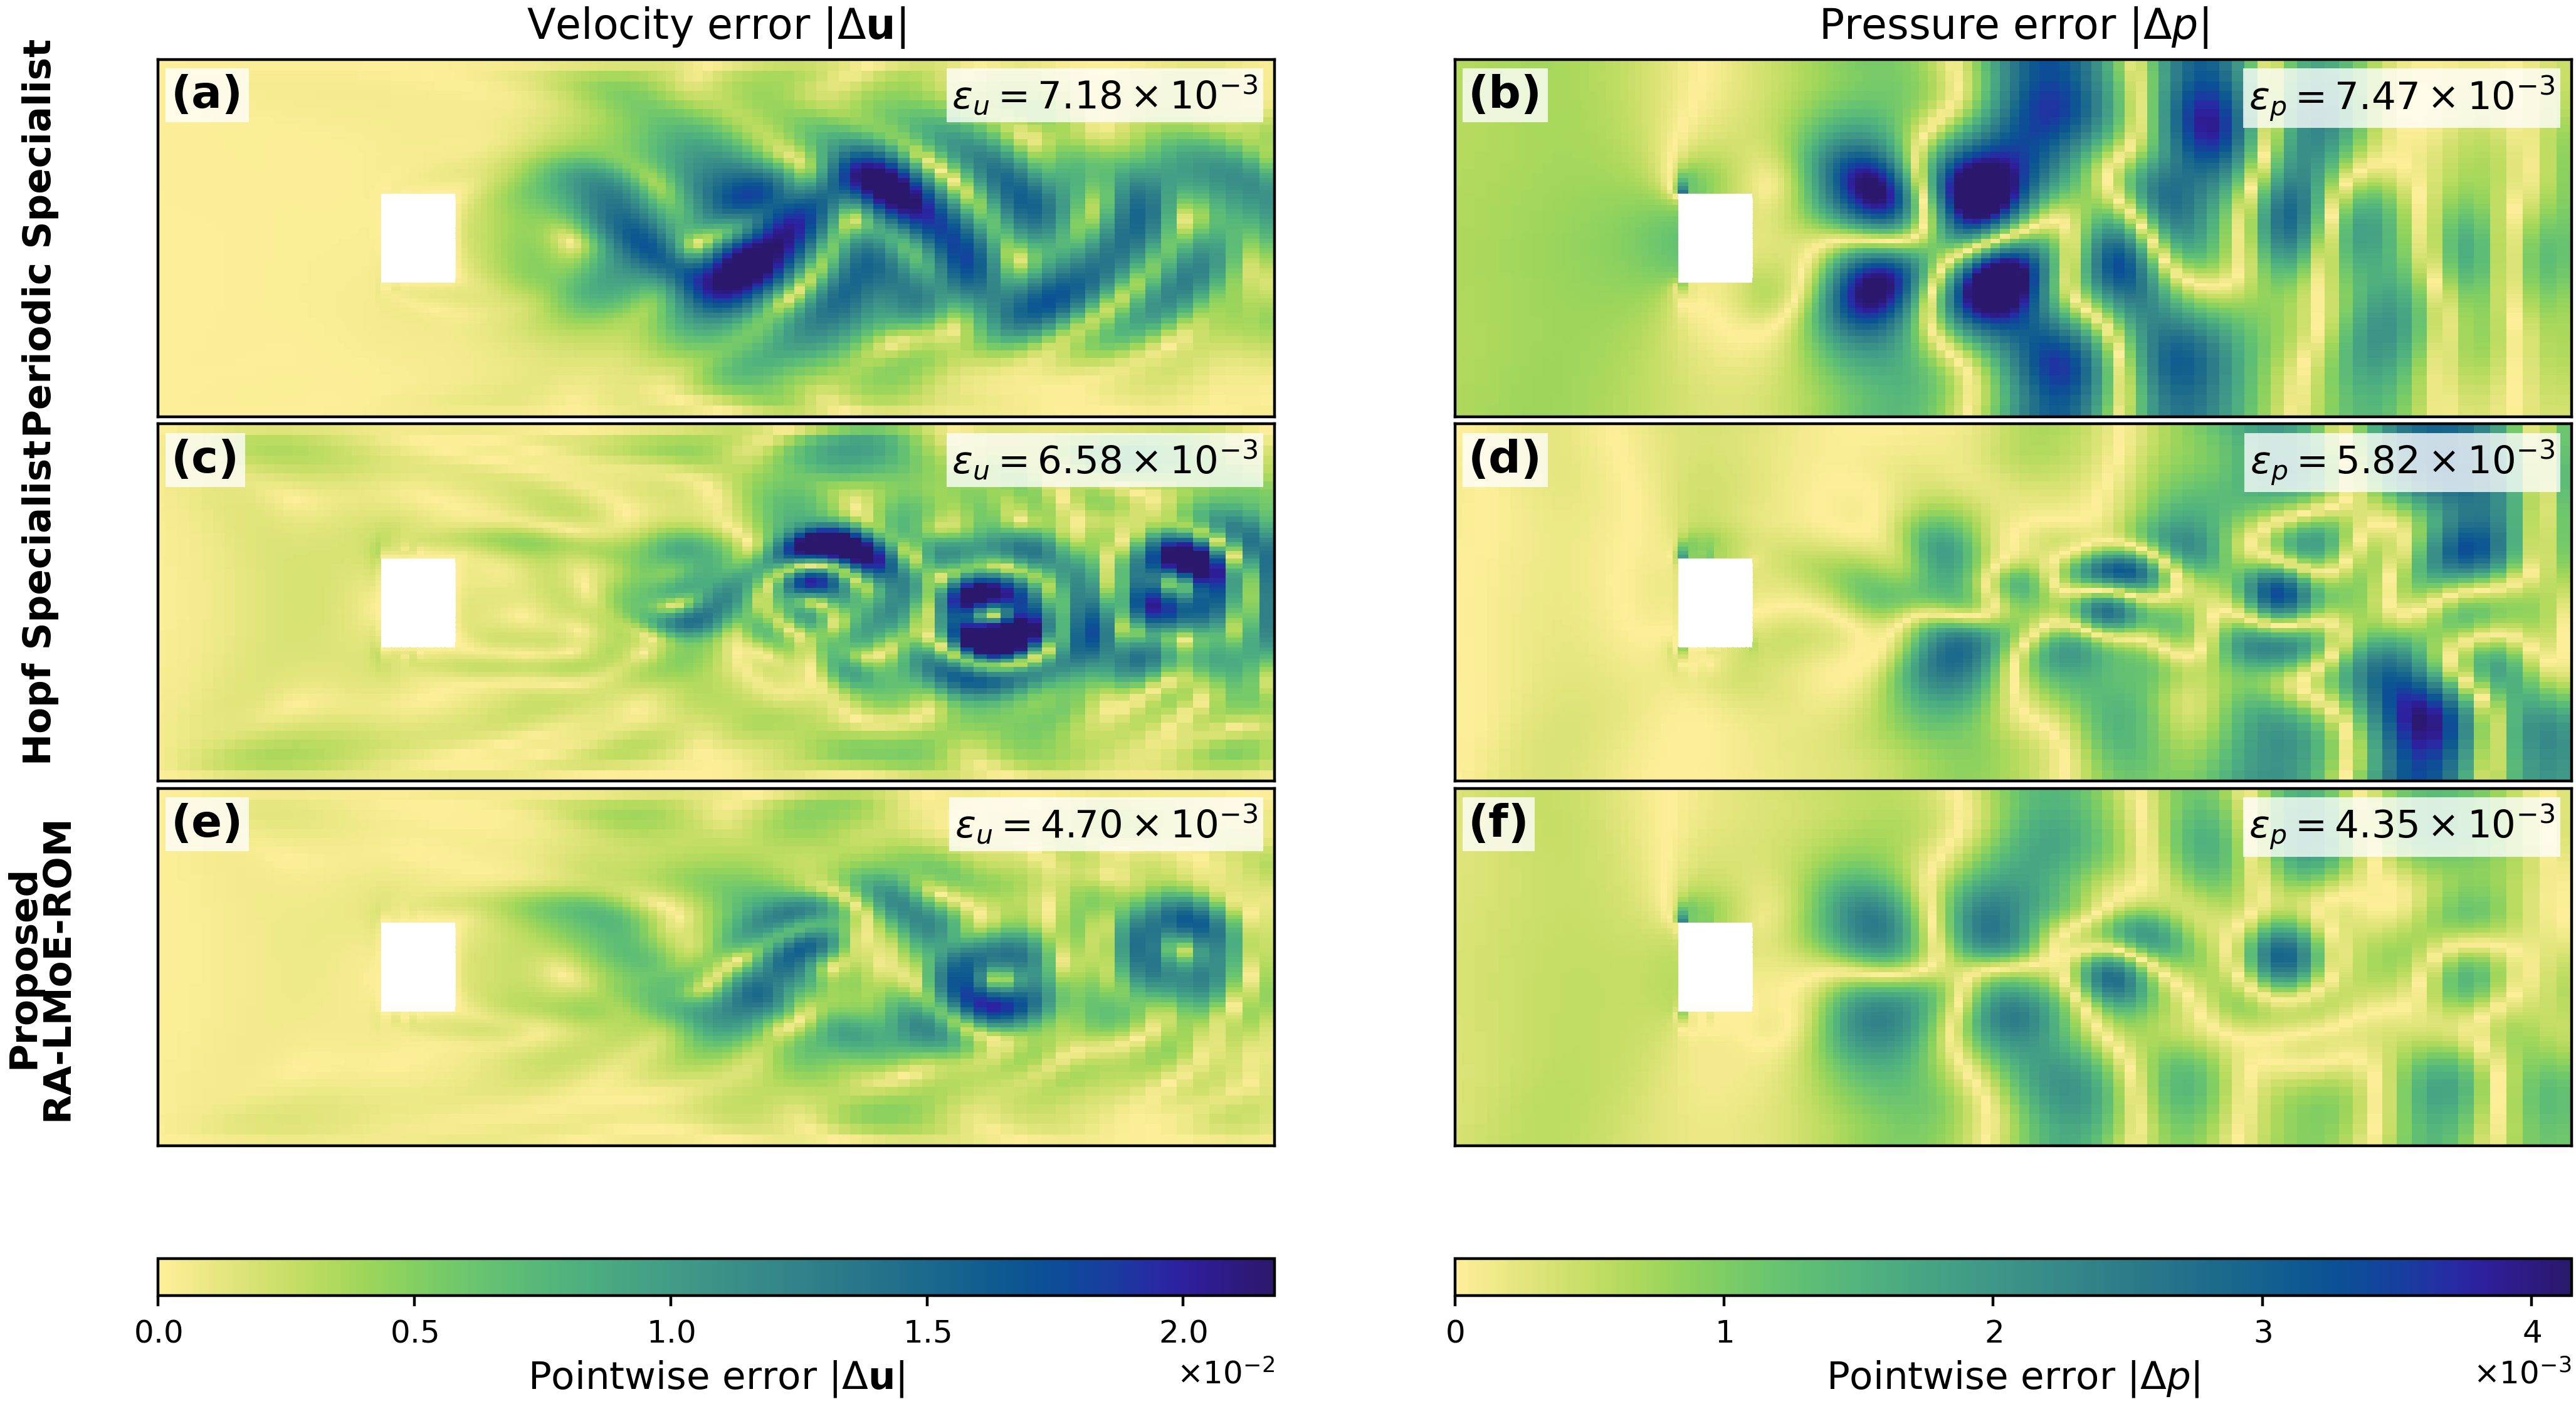
\includegraphics[width=0.80\linewidth]{figures/original/HP_2_1.png}
\caption{Representative held-out prediction in the centered-square
$H$--$P$ overlap at $Re=100.5$. The upper panel compares the CFD reference,
Periodic specialist, Hopf specialist, and T2-C prediction for velocity
magnitude and gauge-corrected pressure. The lower panel gives the
corresponding pointwise absolute errors.}
\label{fig:app_square_hp_full}
\end{figure}
